%
% elemente.tex -- 
%
% (c) 2018 Prof Dr Andreas Müller, Hochschule Rapperwil
%
\subsection{Lineare Differentialgleichungen\label{subsection:lindgl}}
Für eine lineare Differentialgleichung ist die Funktion $f(x)$ linear
in $x$.
Sind $x_1(t)$ und $x_2(t)$ Lösungen der Differentialgleichung
für Anfangswerte $x_1(0)$ und $x_2(0)$, dann ist
$x_1(t)+x_2(t)$ eine Lösung der Differentialgleichung für die
Anfangsbedingung $x_1(0)+x_2(0)$.

\begin{figure}
\centering
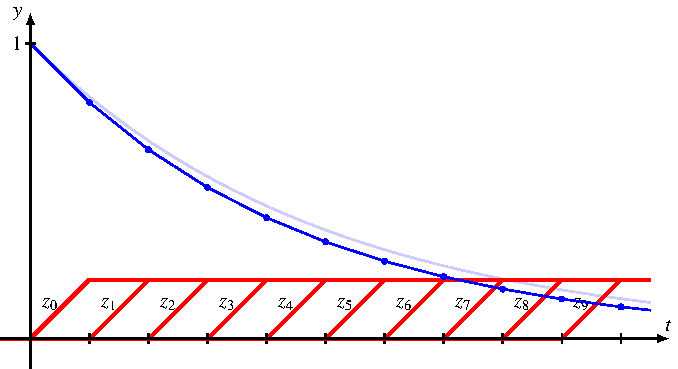
\includegraphics{chapters/3/slopes.pdf}
\caption{Basisfunktionen, aus denen die interpolierte Lösung $\tilde{x}(t)$
durch Linearkombination gefunden werden kann.
\label{skript:elemente:slopes}}
\end{figure}

Die Linearität ermöglicht also, Lösungen der Differentialgleichung
als Linearkombination von Lösungen zu finden.
Das Euler-Verfahren hat diskrete Werte $x_k=x(hk)$ gefunden,
die Werte $x(t)$ für $t$ zwischen den Punkten $t_k=hk$ können
durch Interpolation gefunden werden, wir nennen diese interpolierte
Funktion $\tilde{x}(t)$.
Für einen Punkt $t$ zwischen $t_k$ und $t_{k+1}$ ist dann
\[
\tilde{x}(t) = x(t_k) + (t-t_k) f(x_k, t_k).
\]
Dies kann man auch als Linearkombination von Funktionen
schreiben.
Wir betrachten die Funktionen
\[
z_k(t)
=
\begin{cases}
0&\qquad t < t_k\\
t-t_k&\qquad t_k \le t < t_{k+1}\\
h&\qquad t_{k+1} < t,
\end{cases}
\]
wie sie in Abbildung~\ref{skript:elemente:slopes} rot dargestellt sind.
Damit wird die interpolierte Funktion zu einer Linearkombination:
\[
\tilde{x}(t)
=
x_0 + f(x_0)\cdot z_0(t) + f(x_1)\cdot z_1(t) + f(x_2) \cdot z_2(t) + \dots
=
x_0
+
\sum_{k=0}^n f(x_k) z_k(t).
\]
Diese Lösung ist in Abbildung~\ref{skript:elemente:slopes} blau dargestellt.
Hellblau ist die exakte Lösung $y=e^{-x}$.
Die Lösung $\tilde{x}(t)$ ist also eine Linearkombination
\[
\tilde x(t) = x_0 + \sum_{k=0}^\infty a_k\cdot z_k(t)
\]
der Funktionen $z_k(t)$ schrieben können.
Wir brauchen nur eine Methode, mit der die Koeffizienten $a_k$ bestimmt
werden können.
Da die Funktionen $y_k$ linear sind, könnten wir $\tilde{x}(t)$ in die 
Differentialgleichung einsetzen:
\begin{equation}
\sum_{k=0}^\infty
a_k\frac{d\tilde{z}_k(t)}{dt}
=
f(x_0) + \sum_{k=0}^\infty z_k(t) f(a_k).
\label{skript:elemente:eingesetzt}
\end{equation}
Leider funktioniert das nicht, weil die Funktionen $z_k$ nicht differenzierbar
sind.
Sie sind aber rechtseitig differenzierbar, der Grenzwert
\[
\lim_{\Delta t \to 0+} \frac{z_k(t+\Delta t)-z_k(t)}{\Delta t}
=
\begin{cases}
0&\qquad t<t_k\\
1&\qquad t_k\le t< t_{k+1}\\
0&\qquad t_{k+1} \le t
\end{cases}
\]
existiert immer.
Wenn wir in der Gleichung also überall mit rechtsseitigen Ableitungen
arbeiten, dann bleiben in \eqref{skript:elemente:eingesetzt} an den
Punkten $t_j$ nur wenige Terme übrig.
Auf der linken Seite steht
\begin{equation}
\sum_{k=0}^\infty
a_k\frac{d\tilde{z}_k(t_j)}{dt}
=
a_j,
\label{skript:elemente:links}
\end{equation}
auf der  rechten
\begin{equation}
f(x_0) + \sum_{k=0}^\infty z_k(t_j) f(a_k)
=
f(x_0) + \sum_{k=0}^{j-1} hf(a_k)
=
f\biggl(x_0 + \sum_{k=0}^{j-1} ha_k\biggr).
\label{skript:elemente:rechts}
\end{equation}
Zusammen mit \eqref{skript:elemente:links} folgt
\[
\begin{aligned}
a_0 &= f(x_0)                 &&          &    & \\
a_1 &= f(x_0 + ha_0) = f(x_1) &&\text{mit}&x_1 &= x_0 + ha_0\\
a_2 &= f(x_1 + ha_1) = f(x_2) &&\text{mit}&x_2 &= x_1 + ha_1\\
    &\;\;\vdots
\end{aligned}
\]
Die Idee, die Funktion $x(t)$ als Linearkombination $\tilde{x}(t)$
der Funktionen zu approximieren, führt also auf natürliche Weise
auf das Euler-Verfahren.

Diese Idee lässt sich auf auch auf nichtlineare Differentialgleichungen
verallgemeinern.
Die Tatsache, dass $f(x)$ linear ist in $x$ hat die Hemmschwelle etwas
heruntergesetzt, die Lösung als Linearkombination anzusetzen.
Das Euler-Verfahren macht aber keine solche Voraussetzungen.
Das einzige, was sich ändert, wenn $f(x)$ nicht mehr linear ist,
ist dass die rechte Seite nach Einsetzen der Linearkombination
etwas komplizierter wird.

Dies motiviert ein ganz allgemeines Verfahren zur Lösung von
Diffentialgleichungen:
\begin{enumerate}
\item Wähle eine Familie von Funktionen $z_k(t)$ und setze die Lösung
als Linearkombination
\[
\tilde{x}(t) = \sum_{k=0}^\infty a_k\cdot z_k(t), \qquad a_k\in\mathbb R^n
\]
an.
\item Setze den Ansatz $\tilde{x}(t)$ in die Differentialgleichung ein
und leite daraus Gleichungen für die Koeffizienten $a_k$ ab.
\item Die Gleichungen für $a_k$ können unter Umständen sehr schwierig 
zu lösen sein.
Es kann sogar sein, dass die Gleichungen überbestimmt sind, dass die
$a_k$ also nur zum Beispiel im Sinne der kleinsten Quadrate bestimmt
werden können.
\end{enumerate}
In Abschnitt \ref{section:pdeloesungen} wird diese Idee weiterentwickelt
und gezeigt, wie sie für geeignetere Familien von Funktionen als die $z_k(t)$
erfolgreich sein kann.


